\documentclass[10pt,fleqn]{article}

\usepackage[english]{babel}
\usepackage[utf8x]{inputenc}
\usepackage{enumerate}
\usepackage{amsmath}
\usepackage{amssymb}
\usepackage{amsfonts} 
\usepackage{mathtools}
\usepackage{graphicx}
\usepackage{bm}
\usepackage[usenames,dvipsnames]{color}
\usepackage{todonotes}
\usepackage{dsfont}
\usepackage{hyperref}
\hypersetup{
    colorlinks,
    citecolor=black,
    filecolor=black,
    linkcolor=black,
    urlcolor=black
}
\usepackage{algorithm}
\usepackage{algorithmic}
\usepackage{appendix}
\usepackage{subcaption}
\usepackage{fancyvrb}
\usepackage{subfigure}
\usepackage{graphicx,xcolor}
\usepackage{pifont,mdframed}
\usepackage{tikz}
\usepackage{bm}
\usetikzlibrary{fit,positioning}


%
% Macros
%
\newcommand \cashort[1] { {\todo[color=yello]{#1 -- Cedric}} }
\newcommand \calong[1]  { { \todo[inline,color=yellow]{#1 -- Cedric} } }
\newcommand \gbshort[1] { {\todo[color=cyan!40]{#1 -- Guillaume}} }
\newcommand \gblong[1]  { { \todo[inline, color=cyan!40]{#1 -- Guillaume} } }
\newcommand \mgshort[1] { {\todo{#1 -- Mark}} }
\newcommand \mglong[1]  { { \todo[inline]{#1 -- Mark} } }
\newcommand \bfshort[1] { {\todo[color=green!40]{#1 -- Bryan}} }
\newcommand \bflong[1]  { { \todo[inline,color=green!40]{#1 -- Bryan} } }


% Adds a plus const to the end of a math expression
\def \pcst{+\text{const}}

% A fancy version for capital R
\def \Rcal{\mathcal{R}}

% A fancy version for r
\def \rcal{\mathbf{r}}

% Loss function / log likelihood as appropriate
\def \L{\mathcal{L}}

% KL divergence [Math Mode]
\newcommand{\kl}[2] {
	\text{KL}\left[#1||#2\right]
}

\newcommand \vecf[1] {
    \text{vec}\left(#1\right)
}

\newcommand \ent[1] {
    \text{H} \left[ #1 \right]
}

\newcommand \mut[2] {
    \text{I} \left[ #1 ; #2 \right]
}

\newcommand \dvi[2] {
    \text{D}_\text{VI} \left[ #1; #2 \right]
}

% Starts an expected value expresses [Math Mode]
\newcommand{\starte}[1] {%
	\mathbb{E}_{#1}\left[
}

% Ends an expected value expression [Math Mode]
\def \ende{\right]}

% Starts an varianc expresses [Math Mode]
\newcommand{\startv}[1] {%
	\mathbb{V}\text{ar}_{#1}\left[
}

% Ends an variance expression [Math Mode]
\def \endv{\right]}

%\newcommand \ex[2] {
%    \bigl\langle #1 \bigr\rangle_{#2}
%}
\newcommand \ex[2] {
    \mathbb{E}_{ { #2 } }\left[ #1 \right]
}
\newcommand \var[2] {
    \mathbb{V}ar_{ { #2 } }\left[ #1 \right]
}

\newcommand \halve[1] {
	\frac{#1}{2}
}

\newcommand \half {
    \halve{1}
}

\newcommand \tr { \text{tr} } 

\newcommand \T { ^\top } 

\newcommand \fixme[1] {
    {\color{red} FIXME: #1}
}

\newcommand \vv[1] { \bm #1 }

\newcommand{\mbeq}{\overset{!}{=}}

\newcommand \diag[1] { \text{diag} \left( {#1} \right) }
\newcommand \diagonal[1] { \text{diagonal} \left( {#1} \right) }

\newcommand \Ed {{ \vv{\xi}_d}}
\newcommand \Edj {{\xi_{dj}}}
\newcommand \Edk {{\xi_{dk}}}
\newcommand \AEdj {{\Lambda(\xi_{dj})}}
\newcommand \AEdk {{\Lambda(\xi_{dk})}}
\newcommand \AEd  {{ \bm{\Lambda}(\bm{\xi}_d) }}

\newcommand \Axi { { \Lambda_{\xi} } }
\newcommand \bxi { { \vv{b}_{\xi} } }
\newcommand \cxi { { c_{\xi} } }


\newcommand \wdoc      { { \vv{w}_d } }
\newcommand \wdt[0]  { { w_{dt} } }
\newcommand \wdn[0]  { { \vv{w}_{dn} } }
\newcommand \wdnt[0]  { { w_{dnt} } }
\newcommand \wdd[0]   { { \vv w_{d} } }
\newcommand \zd[0]   { { \vv z_{d} } }
\newcommand \zdn[0]  { { \vv{z}_{dn} } }
\newcommand \zdnk[0] { { z_{dnk} } }
\newcommand \zdk[0]  { { z_{dk} } }
\newcommand \thd[0]  { { \vv \theta_d } }
\newcommand \thdk[0] { { \theta_{dk} } }
\newcommand \thdj[0] { { \theta_{dj} } }
\newcommand \epow[1] { { e^{#1} } }
\newcommand \pkt     { { \phi_{kt}  } }
\newcommand \pk      { { \vv \phi_k } }
\newcommand \lmd     { { \vv \lambda_d } }
\newcommand \lmdk    { { \lambda_{dk} } }
\newcommand \xd      { { \vv x_d } }
\newcommand \atxd     { A ^\top \bm x_d}
\newcommand \axd     { A\bm x_d}
\newcommand \tsq      { { \tau^2 } }
\newcommand \ssq      { { \sigma^2 } }
\newcommand \tmsq     { { \tau^{-2} } }
\newcommand \asq      { { \alpha^2 } }
\newcommand \amsq     { { \alpha^{-2} } }
\newcommand \sgsq     { { \sigma^2 } }
\newcommand \xvec     { { \vv{x} } }
\newcommand \omk      { { \bm \omega _k } }
\newcommand \omkt     { { \omega_{kt} } }
\newcommand \oma     { { \Omega_A } }
\newcommand \gdn      { { \vv{\gamma}_{dn} } }
\newcommand \gdnk     { { \gamma_{dnk} } }
\newcommand \gdk      { { \gamma_{dk} } }
\newcommand \isigt   { { \Sigma^{-1}_{\bm \theta} } }




\newcommand \halfSig { \frac{1}{2\sigma^2} }

\newcommand \nor[2]   { \mathcal{N} \left( {#1}, {#2} \right) }
\newcommand \nord[3]   { \mathcal{N}_{#1} \left( {#2}, {#3} \right) }
\newcommand \mnor[3]  { \mathcal{N} \left(#1, #2, #3\right) }
\newcommand \norp[3]  { \mathcal{N} \left(#1; #2, #3\right) }
\newcommand \mnorp[4] { \mathcal{N} \left(#1; #2, #3, #4\right) }
\newcommand \mul[1]   { \mathcal{M} \left( {#1} \right) }
\newcommand \muln[2]  { \mathcal{M} \left( {#1},{#2} \right) }
\newcommand \dir[1]   { \mathcal{D} \left( {#1} \right) }
\newcommand \pois[1]  { \mathcal{P} \left( {#1} \right) }
\newcommand \gp[2]    { \mathcal{GP} \left( {#1}, #2 \right) }
\newcommand \dir[1]   { \mathcal{D} \left( {#1} \right) }
\newcommand \gam[2]   { \mathcal{G} \left( {#1}, {#2} \right) }
\newcommand \beta[1]  { \mathcal{B}eta \left( {#1}, {#2} \right) }

\newcommand \lne[1]  { { \ln \left( 1 + e^{ #1 } \right) } }
\newcommand \Tr[1]   { \tr \left(  {#1}  \right) }

\newcommand \roud  { \vv{\rho}_{d}  }
\newcommand \rodk { \rho_{dk} }

\newcommand \exA[1]  { \ex{#1}{q(A)} }
\newcommand \exV[1]  { \ex{#1}{q(V)} }
\newcommand \exT[1]  { \ex{#1}{q(\Theta)} }
\newcommand \extd[1] { \ex{#1}{q(\thd)} }
\newcommand \exTV[1] { \ex{#1}{q(\Theta)q(V)} }

\newcommand \Real[0]  { { \mathbb{R} } }
\newcommand \VReal[1] { { \mathbb{R}^{#1} } }
\newcommand \MReal[2] { { \mathbb{R}^{#1 \times #2} } }
\newcommand \Nat[0]  { { \mathbb{N} } }
\newcommand \VNat[1] { { \mathbb{N}^{#1} } }
\newcommand \MNat[2] { { \mathbb{N}^{#1 \times #2} } }

\newcommand \inv[1] { {#1}^{-1} }
\newcommand \invb[1] { \inv{\left( #1 \right)} }

\newcommand \cn { \textsuperscript{\texttt{[{\color{blue}Citation Needed}]}} }

\newcommand \const { { \text{c} } }

\providecommand \floor [1] { \left \lfloor #1 \right \rfloor }
\providecommand \ceil [1] { \left \lceil #1 \right \rceil }


\newcommand \vt[2] { { #1^{(#2)} } }

\newcommand \hashtag[1] { { \ttfamily \##1 } }

\newcommand \mvy  { \vv{m}_{\vv{y}} }
\newcommand \sigvy { { S_Y } }

\newcommand \mmy  { M_Y      }
\newcommand \md   { \vv{m}_d }
\newcommand \phin { \vv{\phi}_n }
\newcommand \isigma { { \inv{\Sigma} } }

\newcommand \sigv     { { \Sigma_V } }
\newcommand \isigv     { { \Sigma^{-1}_V } }

\newcommand \sigy { { \Sigma_Y } }
\newcommand \isigy { { \Sigma_{-1}_Y } }


\newcommand \omy  { { \Omega_Y } }
\newcommand \iomy { { \inv{\Omega_Y} } }

\newcommand \siga     { { \Sigma_A } }
\newcommand \isiga     { { \Sigma^{-1}_A } }
\newcommand \diagv { { \diag{\nu_1,\ldots,\nu_P} } }

\newcommand \ma { \vv{m}_a }
\newcommand \my { \vv{m}_y }

\newcommand \VoU { V \otimes U }

\newcommand \one { \mathbb{1} }
%\newcommand \one  {{  \mathds{1} }}

\newcommand \lse { \text{lse} }
%\newcommand \lse[0] { \mathrm{lse} }

% Conditional independence 
\def\ci{\perp\!\!\!\perp} % from Wikipedia



% ------ For the eval section

% Multinomial PDF [Math Mode]
% params: 1 - the variable
%         2 - the value
%         3 - the state indicator (e.g. k for a distro with K values)
%         4 - any additional subscript
\newcommand{\mpdf}[4] {
	\prod_{#3} {#1}_{{#4} {#3}} ^ {#2}
}

% Dirichlet PDF [Math Mode]
% params: 1 - the variable
%         2 - the hyper-parameter
%         3 - the state indicator (e.g. k for a distro with K values)
%         4 - any additional subscript
\newcommand{\dpdf}[4] {
	\frac{1}{B({#2})} \prod_{#3} {#1}_{{#4} {#3}} ^ {({#2}_{#3} - 1)}
}

% To simplify the sampling equations, this is indicates
% that the given value has had datapoint "m" stripped out
%
\newcommand{\lm}[1] {
	#1^{\setminus m}
}

\newcommand \model[0] {
    \mathcal{M}
}

\newcommand \perplexity[1] {
    \mathcal{P} \left( { #1 } \right)
}

\newcommand \WTrain {
    \mathcal{W}^{(t)}
}

\newcommand \WQuery {
    \mathcal{W}^{(q)}
}

\newcommand \oneover[1] {
    \frac{1}{ {#1} }
}

\newcommand \samp[1] {
    { #1 }^{(s)}
}

\newcommand \etd[0] {
    \vv{\eta}_d
}

\begin{document}



\section{Multi-Task Prediction of Admixture Components for Microtexts}
Bayesian admixture models have recently proved popular, particularly relative to traditional mixture models, as a means of modelling observations. Admixture models allow large numbers of mixing components without the over-fitting which would typically affect unregularlized mixture models. Moreover they provide an easily interpretable mechanism for dimensionality reduction.

While predated by other work\cite{Pritchard2000} the most popular instance of admixture models in use is the Latent Dirichlet Allocation (LDA) algorithm\cite{Blei2003} which is typically applied to textual corpora. In LDA each document is described by a mixture drawn from a Dirichlet distribution, from which per-token mixture assignments are sampled. The individual mixture components are typically referred to as ``topics" in this case, and the family of admixture-models for text typically referred to as ``topic-models"

A disadvantage of LDA is that it does not adequately capture correlations between mixture components. An alternative is the Correlated Topic Model (CTM) where the Dirichlet prior over mixture components is replaced with a Normal distribution, whose covariance captures correlations between components, with a logistic-link function used to translate these mixture-component strengths into a probability distribution.\cite{Blei2006}. CTM has been shown to out-perform LDA -- according to held-out likelihood -- for a fixed number of mixture components, however the resulting topics are less interpretable\cite{Chang2009}. Other approaches to capturing topic-correlation include Supervised LDA\cite{Rubin2011}, which embeds within the LDA framework another LDA model over mixture-components themselves, Pachinko allocation \cite{Li2006} which uses a form of multinomial PCA\cite{Buntine2002} to learn a low-rank representation of ``intermediate" topics, and independent factor models\cite{Putthividhya2009} which learnt a low rank form of the covariance over topics in the CTM model.

Both LDA and CTM rely on token co-occurrences in documents, and so have shown poor performance when applied to micro-texts such as individual tweets from Twitter\cite{DeLaRosa2011} where the document size is very small (e.g. 13 words) and much smaller than the number of topics (e.g. $K=100$) learning to an overparameterised model. More successful approaches have involved grouping tweets a-priori, for example by author\cite{Weng2010}\cite{Xu2011}\cite{Hong2010}\cite{Eisenstein2010} and then applying LDA to that group, an approach referred to a the ``author-topic model"\cite{MacCallum2007}. A disadvantage of this approach however is that that not all tweets' topics may be attributable to a single variable -- in this case, author. A simple approach to this was used in \cite{Xu2011} where a bernoulli switch is used to determine whether a tweet is attributable to an author's long-term interests or not. Inference was performed in the former case, and ignored in the latter case, so as to characterise authors better. 

Such an approach is unsatisfying when modelling micro-text corpora - clearly an individual tweet's topics depend on a variety of factors: the author's long-term interests; interests globally popular at a particular time, such as news events; the author's location and others. Were one to jointly consider all these features, one might obtain a tighter model fit. There are many special case topic models dealing with documents modelled alongside author\cite{RosenZvi2004}, time\cite{Wang2006}, and geography\cite{Eisenstein2010}; however while one could combine such models, it would be preferable to have a single model which could take any features/words matrix pair and perform inference. Such an approach could be applied to many more use-cases, such as image-labelling.

One such model is Dirichlet Multinomial Regression (DMR)\cite{Mimno2008}. In this model, separate weight vectors are learned for each mixture-component, and then used to predict the individual component-strengths for all topics. These are then combined into a vector used to parameterise the Dirichlet distribution from which the component-mixture for an individual document (or other observation) can be sampled. 

A weakness of DMR however is precisely that it predicts each component-strength independently of all other components. Considering the advantages that CTM has over LDA, it seems sensible to view it as a multi-task learning problem, where we capture correlations between features and between individual tasks -- in this case corresponding to component mixture-strengths. By sharing information between these component-prediction tasks one can improve performance over the no-sharing case. Multi-task learning has been shown to provide a better fit compared to learning tasks individually\cite{Archambeau2011}\cite{Argyriou2008}, though only where task or feature correlations exist which can be exploited\cite{Caruana1997}. It should be noted that DMR, if viewed as predicting individual word-counts, is technically a multi-task learning algorithm, as it transfers knowledge between tasks (word-counts) by learning a low-rank representation over the labels -- the topics.

In this paper we present a model for predicting mixture-components in an admixture model. We learn a single matrix which we use to predict all mixture components from a given weight vector, exploiting correlations between mixture components. By use of appropriate matrix-variate priors, we additionally learn a shared covariance matrix over mixture-components and a low-rank covariance over features. We demonstrate the performance of this model on multiple real-world datasets.

\subsection{The Matrix-Variate Normal Distribution}
A matrix $A \in \MReal{K}{F}$ which has a matrix-normal distribution\cite{Gupta1999} with row-covariance $\Omega \in \MReal{F}{F}$, column covariance $\Sigma \in \MReal{K}{K}$ and mean-matrix $M \in \MReal{K}{F}$ has the density:

\begin{equation}
p(W) = (2\pi)^{KF}|\Sigma|^{-F}|\Omega|^{-K} \exp\left(\half \inv{\Sigma}\left(A - M\right) \inv{\Omega} \left(A - M \right)\T\right)
\end{equation}

It is related to the multivariate normal distribution by the identity $\mnor{M}{\Omega}{\Sigma} = \nor{\vecf{M}}{\Sigma \otimes \Omega}$ where $\vecf{\cdot}$ is the function that converts a matrix to a vector by stacking its columns. 

The row and column covariances $\Omega$ and $\Sigma$ are unidentifiable as $ A \otimes B = \lambda A \otimes \frac{1}{\lambda}B$ for any scalar $\lambda$. In practice this is resolved by forcing last element on the diagonal of one of the matrices to 1, giving rise to the iterative ``flip-flop" algorithm \cite{Srivastava2009} in the maximum-likelihood setting, or by appropriate selection of priors\cite{Archambeau2011}\cite{Yang2011}.

The use of matrix-variate priors for multitask learning has been explored in \cite{Stegle2011}\cite{Bonilla2008} \cite{Archambeau2011}\cite{Yang2011}. Due to the ability to reduce the number of covariance parameters from $(LF)^2$ to $L^2 + F^2$ it has also been explored in other areas such as matrix factorization\cite{Allen2010}.

\subsection{Multitask Multinomial Regression}
Let $D$ be the number of documents and $N_d$ the number of words in document $d\in\{1,\ldots,D\}$. The Correlated Topic Model models the mixture $\thd$ for a document $d$ as follows:
\begin{align}
\thd &\sim \nor{\mu}{\Sigma}
&\zdn | \thd &\sim \muln {\vv{\sigma}(\thd)}{1} ,\\
\pk &\sim\dir{\vv{\beta}}
&\wdn | \zdn , \{\pk\}_k &\sim \muln{\vv{beta}_{\zdn}}{1}
\end{align}
where $\vv{\sigma}(\thd) = \{\sigma_1(\thd), \ldots, \sigma_k(\thd)\}$; $\sigma_k(\thd) = \exp(\thdk - \lse(\thd))$ is the multivariate softmax function; and $\lse(\thd) = \ln\left(\sum_j \thdj \right)$ is the log-sum-exp function. The latent variable $\zdn$ is the mixture-component assignment for the n-th token in document $d$ stored as a 1-of-K vector. Similarly, the corresponding token is identified by the 1-of-T vector $\wdn$. The mixture distribution for the k-th mixture is given by the vector $\vv{\beta}_k$ which we treat as a parameter.

In our model we specify the mixture-distribution for a document $d$ as a linear combination of the that documents feature-vector $\xd \in \VReal{F}$ by means of a matrix $A \in \MReal{K}{F}$.
\begin{align}
Y \sim & \mnor{0}{\rho^2 I_P}{\Sigma} & A|Y \sim & \mnor{YV}{\alpha^2 I_F}{\Sigma} \\
\thd | A \sim & \nor{\axd}{\Sigma}
\end{align}

where $\Sigma$ is the covariance over topics and the matrix $V \in \MReal{P}{F}$ projects from a low-rank feature-space to the observed feature-space. The rest of the model follows as with CTM. By converting to multi-variate normal form, and employing the usual marginal normal identity\cite{Bishop2006}  we can see that the marginal distribution of $A$ is
\begin{equation}
A \sim \mnor{0}{\alpha^2 I_F + \rho^2 V\T V}{\Sigma}
\end{equation}

where the low-rank decomposition of the covariance over features is clear. We refer to this as the \emph{full-covariance model}, as it stores a full-rank representation of the covariance over mixture-components. It should be noted that such marginalisations are only possible if both distributions share one covariance matrix, which is why we tie the component-covariances over the distributions over Y, A and $\thd$

It is interesting to note that were we to use the distribution $A \sim \mnor{0}{\alpha^2 I_F}{\Sigma}$ and then marginalize out A from the distribution of $\thd$ we would obtain the multi-task Gaussian Process regression algorithm of \cite{Bonilla2008}. In this context, the resulting model would provide a correlated-topic analogue to the Kernelised Topic Model \cite{Hennig2012} which makes the LDA assumption of topic independence. Like KTM however, it would be challenge to scale to large corpora with large numbers of topics.

\subsubsection{Variational Inference}
%\newcommand \Axi { \Lambda_{\xi_d} }
%\newcommand \bxi { \vv{b}_{\xi_d} }
%\newcommand \cxi { \vv{c}_{\xi_d} }
%\newcommand \lse[1] { \text{lse}\left(#1\right) }
\newcommand \onek { \one_K }
\newcommand \md { \vv{m}_d }
\newcommand \Vd { V^{(d)} }


\newcommand \sigmoid[1] { {  \vv{\sigma}\left( #1 \right)  } }
\newcommand \sigmoidk[1] { {  \sigmoidat{#1}{k}  } }
\newcommand \sigmoidat[2] { {  \sigma_{#2}\left( #1 \right)  } }
\newcommand \ged { { \nabla_{\Ed} } }
\newcommand \gesig { { \ged \left[ \sigmoid{\Ed} \right] } }

First we consider the full-covariance model. We use the standard EM framework to estimate the latent variables $\{Y, A, \thd, \zdn\}$ and and maximise parameters $\Sigma$, $V$ and $\vv{\beta}_k$ for $k \in 1\ldots K$. As the posterior is intractable, we employ the mean-field approximation $q(Y, A, \Theta, Z) = q(Y)q(A)q(\Theta)q(Z)$. 

\begin{align}
q(Y) = & \mnor{M_Y}{R_Y}{S_Y} & q(A) = & \mnor{M_A}{R_A}{S_A} \\ 
q(\Theta) = & \prod_d \nor{\md}{\Vd} & q(Z) = & \prod_d \prod_n \muln{\vv{\gamma}_{dn}}{1} 
\end{align}


Where $\Vd$ is a diagonal matrix in all our experiments.

\subsubsection{Resolving Identifiability in the Matrix-Variate Posterior}
Taking derivatives of the free-energy and setting to zero in the usual manner initially leads to the following updates for $R_Y$ and $S_Y$.

\begin{align}
P \times \inv{S_Y} = & \inv{\Sigma}\Tr{\rho^2 I_P R_Y} + \inv{\Sigma}\Tr{\alpha^2 V V\T R_Y} \\
\implies S_Y = & \frac{\Tr{\left(\rho^{-2} I_P + \alpha^{-2} V V\T\right) R_Y}}{P} \Sigma \\ 
R_Y = & \frac{\Tr{\inv{\Sigma}S_Y}}{K} \invb{\rho^{-2} I_P + \alpha^{-2} V V\T}\end{align}

Substituting the value for $R_Y$ into the update for $S_Y$ we obtain

\begin{align}
S_Y = \frac{\Tr{\inv{\Sigma}S_Y}}{K} \Sigma
\end{align}

Premultiplying both sides by $\inv{\Sigma}$ we see that
\begin{align}
\inv{\Sigma} S_Y = \frac{\Tr{\inv{\Sigma}S_Y}}{K} I_K
\end{align}

Implying that the product $\inv{\Sigma} S_Y$ is a scalar multiple of the identity matrix, and therefore $S_Y = \{ q \Sigma | q \in \Real, q \neq 0 \}$ where the inequality arises from the assumption that an inverse must exist. This -- coupled with the equivalent trace term in the update for $R_Y$ -- is simply a manifestation of the Kronecker identifiability issue mentioned earlier. If we set q = 1 in this case and substitute $S_Y$ into the update for $R_Y$ we obtain the considerably simpler equations:

\begin{align}
S_Y = & \Sigma &
R_Y = & \invb{\rho^{-2} I_P + \alpha^{-2}V V\T}
\end{align}

No such special treatment is required to obtain the update for $M_Y$

\begin{align}
M_Y = & \invb{\rho^{-2} I_P + \alpha^{-2} V V\T}(\alpha^{-2}V M_A) = R_Y (\alpha^{-2} V M_A)
\end{align}

The updates for the posterior $q(A)$ follow similarly.

\subsubsection{Non-Conjugate Inference with Quadratic Bounds}
Our posterior is still intractable however as the multinomial distribution over per-token topics $Z$ is not conjugate to the normally distributed prior.

To overcome this we bound the log-sum-exp function with a quadratic function of its arguments, which allows for closed-form updates in the E-Step and M-Step. 
\begin{align}
\lse(\thd) & \leq \half \thd\T \Axi \thd - \bxi\T\thd + \cxi
\end{align}

We consider two possible quadratic bounds. First we consider the Bouchard bound\cite{Bouchard2007} which bounds the log-sum-exp function as a product of sigmoids, and then uses the Jaakola bound\cite{Jaakkola1997} to further bound the sigmoids in turn, obtaining the bound below.

\begin{align}
\Axi & = 2 \text{diag}_k
    \left(
        \frac{1}{2\Edk}\left(\frac{1}{1 + e^{\Edk}} - \half\right)
    \right) \\
\bxi & = \half I_K - s_d \Axi \\
\cxi & = \half \left( s_d + s_d^2 \Axi \onek\T\onek - \Ed\T\Axi\Ed -  s_d \onek - \Ed\right) + \text{vec}_k\left({\ln 1+e^{\Edk}}\right)
\end{align} 

Next we consider the Bohning bound\cite{Bohning1988}, which takes a second-order Taylor approximation of the log-sum-exp function around a point $\Ed$, then replaces the Hessian $H(\Ed)$ with a matrix $\Lambda$ such that $\Lambda - H(\Ed)$ is positive-definite for all $\Ed$, resulting in the bound below:

\begin{align}
\Axi & = \half \left(I_K - \mathbf{1}_K\mathbf{1}_K\T / K  \right) \\
\bxi & = A \Ed  - \sigmoid{\Ed} \\
\cxi & = \half \Ed\T A \Ed - \sigmoid{\Ed}\T\Ed + \ln(\sum_k e^{\Edk}))
\end{align} 


With this bound, we see that the distribution over Z becomes

\begin{align}
\ln p(Z) = & \sum_d \sum_n \sum_k \zdnk \thdk - \sum_d \sum_n \sum_k \zdnk \lse(\thd) \\
\geq & \sum_d \sum_n \sum_k \zdnk \thdk - \sum_d \sum_n \sum_k \zdnk \left( \half \thd\T A \thd + \bxi\T\thd + \cxi \right)\\
= & \sum_d \sum_n \sum_k \zdnk \thdk - \sum_d N_d \left( \half \thd\T A \thd + \bxi\T\thd + \cxi \right)
\end{align}

In the case of the Bouchard bound, the bound parameters $\Ed, s_d$ are trivially obtained by taking derivatives of the free-energy and setting to zero. For the Bohning bound, taking the derivative with respect to $\Ed$ and setting to zero leads to the following cubic equation:

\begin{align}
\md\T \Axi
- \md\T\gesig
- \Ed \Axi
+ \Ed\T\gesig
+ \sigmoid{\Ed}
- \sigmoid{\Ed}
\mbeq 0
\end{align}
which has a minimum at $\Ed = \md$.

There are other approaches to dealing with non-conjugacy. One approach is to take a Taylor approximation of the posterior around a particular point. If that point is arbitrary, one obtains the method used in the original CTM paper\cite{Blei2003}, if it's around the true mean one obtains the delta-method, as employed in\cite{Teh2007}, and if it's taken around the mode one obtains the usual Laplace approximation\cite{Bishop2006}. These three methods were examined in the case of CTM in\cite{Wang2013a} where the best results were obtained with the Laplace approximation. However all approaches required complex nested inference schemes, with gradient descent and/or Newton-Raphson employed for some variable updates in the overall inference loop.

Equally other bounds to the log-sum-exp function have also been proposed, such as the piece-wise quadratic bound of \cite{Marlin2011} or the ``tilted" bound of \cite{MinkaKnowles} but these too do not admit fast, closed-form inference.

In practice we adapt the model to a back of word-counts $\vv{w}_d \in \VReal{T}$ instead of a list of $N_d$ word observations, and with a matching change from $Z^{(d)} \in \MReal{N_d}{K}$ to $Z^{(d)} \in \MReal{T}{K}$ we use these updates to obtain algorithm \ref{alg:yv}. As it is impossible to store $Z \in \mathbb{R}^{D\times T \times K}$ in memory for any non-trivial problem, we substitute the update for Z into those expressions that employ it and recalculate.

Even with this change, the performance of this algorithm is still quite slow, due to the need to invert a function of the covariance matrix for every update of the posterior mean $\md$. This is particularly problematic for the micro-text example where a small corpus may easily contain millions of ``documents". 

In the case of micro-texts, and the Bohning bound implementation, a simple optimisation is possible. As the matrix $\Axi$ is constant for all documents, the only term that differs from document to document is the document length, $N_d$. For micro-texts, the number of distinct document-lengths is much smaller than the number of documents themselves: indeed in the Twitter corpus introduced in the next section, amongst 750,000 tweets there are less than 50 unique document lengths, distributed as a Poission distribution with mean 10. Therefore the number of matrix inversions can be kept small by pre-generating the posterior-variance for each distinct document length.

This optimisation will not work for standard corpora however, where the number of distinct document lengths may well approach the number of documents; neither will it work in the case of the Bouchard bound, as the $\Axi$ term will differ from document to document. %To address this, we consider a modification of the model in the next section.


\begin{algorithm}
\caption{Representing $A=YV$}
\label{alg:yv}
$\text{ }$\\
{\bf E-Step}
    \begin{align*}
        S_Y = & \Sigma \quad R_Y = & \invb{\rho^{-2} I_P + \alpha^{-2}V V \T}
        \quad M_Y = & R_Y \left( \alpha^{-2} V M_A \right) \\
        S_A = & \Sigma \quad R_A = & \invb{\alpha^{-2} I_F + \sigma^{-2} X\T X} 
        \quad M_A = & \left(\alpha^{-2} YV + \sum_d \md \inv{\Sigma} \xd\T\right)R_A
    \end{align*}
    \begin{align*}
         \Vd = & \invb{\inv{\Sigma} + N_d \Axi} & \text{\emph{In practice we use only the diagonal}}\\
         \md = & \invb{\inv{\Sigma} + N_d \Axi} \left(\inv{\Sigma} M_A \xd  + N_d \bxi + Z^{(d)}\vv{w}_d \right )\\
        \gamma_{dvk} \propto & \beta_{kv} e^{m_{dk}} 
\end{align*}
{\bf M-Step}
\begin{align*}
    V = & \invb{K \times R_Y + M_Y\T \inv{\Sigma} M_Y}M_Y \inv{\Sigma} M_A \\
    \Sigma = & \frac{1}{P+F+D} \left(M_Y M_Y\T + (M_A - Y V)(M_A - Y V)\T \right. \\
        & \qquad \qquad \left. + \sum_d \left[ \Vd + (\md - A \xd)(\md - A\xd)\T \right] \right)\\
     \beta_{kv} \propto & \sum_d z_{dvk} w_{dv} 
\end{align*}
{\bf Bouchard Bound M-Step}
    \begin{align*}
        \Axi & = 2 \text{diag}_k
    \left(
        \frac{1}{2\Edk}\left(\frac{1}{1 + e^{\Edk}} - \half\right)
    \right) \\
\bxi & = \half I_K - s_d \Axi \\
        \Edk = & \sqrt{m_{dk}^2 - 2s_d m_{dk} + s_d^2 + V^{(d)}_{kk}} \\
        s_d = & \frac{\frac{K}{4} - \half + \sum_k m_{dk} \AEdk}{\sum_k \AEdk} \\
    \end{align*}
{\bf Bohning Bound M-Step}
    \begin{align*}
        \Axi & = \half \left(I_K - \mathbf{1}_K\mathbf{1}_K\T / K  \right) \\
        \bxi & = \Axi \md  - \sigmoid{\md}
    \end{align*}
\end{algorithm}

%\subsubsection{Low-Rank Covariance}
%To address the performance issue with the Bouchard algorithm variant, and further to handle the issue of rank-deficient matrices when topic-counts are high, we propose a modification to the algorithm, where we employ a low-rank decomposition of the topic-covariance matrix in addition to the feature-covariance.
%
%To obtain this low-rank covariance we alter the distributions over $Y$, $A|Y$ and $\thd$ as follows:
%
%\begin{align}
%Y \sim & \mnor{0}{\rho^2 I_P}{\tau^2 I_Q} & A|Y \sim & \mnor{UYV}{\alpha^2 I_F}{\sigma^2 I_K} \\
%\thd | A \sim & \nor{\axd}{\sigma^2 I_K}
%\end{align}
%
%Unfortunately, we can no longer obtain a matrix-variate marginal distribution over W, and so must use the multi-variate density to describe the marginal distribution.  
%
%
%\begin{align}
%\vecf{A} \sim \nor{\vv{0}}{\alpha^2 \sigma^2 I_{FK} + \rho^2 V\T V \otimes \tau^2 U U \T}
%\end{align}
%
%We refer to this as the reduced-covariance model.

%\subsection{Inference for the Reduced-Covariance Model}
%One approach to the reduced covariance model is to attempt to use matrix-variate posteriors with separate covariances -- $q(Y) \sim \mnor{M_Y}{R_Y}{S_Y}$, $q(A) \sim \mnor{M_A}{R_A}{S_A}$ --  despite the non-separability of the marginalized prior. However this immediately leads to a Sylvester equation, indicating that the covariance of the variational posterior is non-separable.
%
%\begin{align}
%S_Y = & \frac{1}{P}\invb{\Tr{\rho^{-2} R_Y}\tau^{-2}I_K + \Tr{\alpha^{-2}V V\T R_Y} \sigma^{-2}U\T U } \\
%R_Y = & \frac{1}{Q}\invb{\Tr{\tau^{-2} S_Y}\rho^{-2}I_P + \Tr{\sigma^{-2} U\T U} \alpha^{-2} V V\T} \\
%\vecf{M_Y} = & \invb{\rho^{-2}\tau^{-2} I_{PQ} + \alpha^{-2}V V\T \otimes \sigma^{-2} U \T U}\vecf{\sigma^{-2}\alpha^{-2} U\T M_A V\T}
%\end{align}
%
%The trick employed previously to eliminate the trace terms from the covariances is clearly not possible in this case as there are different scaling factors for the two summands in each case. Moreover, without employing such a trick, or any other constraints as in the flip-flop algorithm, the updates above fail to specify a single identifiable solution for the covariances and so the two estimates may diverge to extremely small and large values respectively, as has been observed in experiments.
%
%
%{\color{red}
%{\bf Viability and Identifiability:}
%
%\begin{enumerate}
%    \item Am I right in saying there is no way of canceling out the traces?
%    \item When I experimented with this model in October ($Y=UYV$, matrix-variate posteriors) I encountered an identifiability issue with the two covariance matrices, which I finally tracked to the Kronecker product. The trick of fixing the final element of the diagonal is described for MLE in \cite{Srivastava2009} but I'm currently struggling to apply it to the VB case. Some of the matrix identities in \cite{Minka2000a} may also be useful.
%    \item I think furthermore that the same trick needs to be employed for U and V to avoid identifiability issues with those matrices as well - is this correct?
%\end{enumerate}}
%
%
%
%Noting that the materialization of a $P^2 \times Q^2$ matrix is unavoidable, we therefore chose to use a multi-variate posterior for Y, $q(\vecf{Y}) = \nor{\vv{m}_y}{S_Y}$ where $\vv{m_y} \in \VReal{P\times Q}$ and $S_Y \in \MReal{(P \times Q)}{(P \times Q)}$, while retaining the matrix-variate prior for A. This formulation, by eschewing the Kronecker product in the covariances, also solves the identifiability issue.
%
%{\color{red}
%However now V and U appear in a Kronecker product so I need to presumably constrain these as well.
%}
%
%This gives rise to the following expectations
%
%\begin{align}
%\ex{p(Y)}{q} = & -\halve{PQ}\left(\ln 2\pi + \ln \rho^2 + \ln \tau^2\right) - \half \left(\rho^{-2}\tau^{-2} \vv{m}_y\T\vv{m}_y + \Tr{\rho^{-2}\tau^{-2} S_Y}\right) \\
%\begin{split}
%\ex{p(A|Y)}{q} = & -\halve{FK}\left(\ln 2\pi + \ln \rho^2 + \ln \tau^2\right) \\
% & -\half \Tr{\alpha^{-2}\sigma^{-2}(M_A - U M_Y V)(M_A - U M_Y V)\T} \\
% & -\half \Tr{S_Y \left(\alpha^{-2}V V\T \otimes \sigma^{-2}U \T U\right)} \\
% & -\half \Tr{\sigma^{-2}S_A\otimes \alpha^{-2}R_A}
% \label{eqn:free_enery_u_and_v}
%\end{split}
%\end{align}
%
%To determine how the covariance of Y should appear in the PDF of X we used the standard identities for the $\vecf{\cdot}$ and kronecker product operators. These are given in the appendix.
%
%\newcommand \mvy  { \vv{m}_{\vv{y}} }
%\newcommand \sigvy { { S_Y } }
%
%\newcommand \mmy  { M_Y      }
%\newcommand \omy  { \Omega_Y }
%\newcommand \sigy { \Sigma_Y }
%
%\subsubsection*{Matrix Calculus for Kronecker Products}
%Solving for $U$ and $V$ requires the use of the vec-transpose \emph{operator} introduced in \cite{Wandell1992} and the \emph {communtation matrix} introduced in \cite{Magnus1988}. These are described here.
%
%The vec-transpose of an $m \times n$ matrix $X$, denoted by $\vt{X}{p}$ is composed of $n$ submatrices stacked atop one another, where each $p \times ^m/_p$ sub-matrix is generated by a fortran-order reshaping of each column of X. The matrices are generated from top to bottom from the columns of X read from left to right. It generalizes both the transpose and $\vecf{\cdot}$ operations, as $\vt{X}{1} = X\T$ and $\vt{X}{\text{rows}(X)} = \vecf{X}$.
%
%For an $m \times n$ matrix X, the commutation matrix is the square permutation matrix $T_{mn} \in \{0,1\}^{(m \times n) \times (m \times n)}$ that transforms $\vecf{X}$ into $\vecf{X\T}$ such that:
%\begin{equation}
%T_{mn} \vecf{X} = \vecf{X\T}
%\end{equation}
%
%With these we can define the following identities for the differentiation of terms in both sides of a Kronecker product. For the purpose of these identities only let $A \in \MReal{a}{nl}$, $X \in \MReal{m}{n}$ and $Y \in \MReal{k}{l}$ and thereby define
%
%\begin{align}
%\begin{split}
%\frac{d}{dX} \Tr{A\T(X\T X \otimes Y\T Y)} & = 2X \left(\vt{A}{l}\right)\T (I_{nl} \otimes Y\T Y) \vt{I_nl}{l} \label{eqn:lhs_kro_derivative_symm}
%\end{split} \\
%\begin{split}
%\frac{d}{dY} \Tr{A\T(X\T X \otimes Y\T Y)} & = 2 Y \left(\vt{(T_{ln} A)}{n}\right)\T (I_{nl} \otimes X\T X ) \vt{\left( T_{ln} \right)}{n} \label{eqn:rhs_kro_derivative_B_is_ident}
%\end{split}
%\end{align}
%
%The vec-transpose operator and the commutation matrix and their applications to calculus are explained in more detail in \cite{Minka2000a}. The appendix provides a summary of the key points, and the derivations of \eqref{eqn:lhs_kro_derivative_symm} and \eqref{eqn:rhs_kro_derivative_B_is_ident}.
%
%\subsubsection*{Derivation of the updates for U and V}
%
%Starting first with V, we can use \eqref{eqn:lhs_kro_derivative_symm} to take the derivative of \eqref{eqn:free_enery_u_and_v} and so derive the following solution
%
%\begin{equation}
%V = \invb{\mmy\T U\T U \mmy + \left(\vt{S_Y}{Q}\right)\T (I_{PQ} \otimes U\T U) \vt{I_{PQ}}{Q} } \sigma^{-2} M_A \T U \mmy
%\end{equation}
%
%Next, for U, we employ \eqref{eqn:rhs_kro_derivative_B_is_ident} which provides the solution:
%\begin{equation}
%U = \invb{\mmy V\T V \mmy\T + \left( \vt{(T_{QP} S_Y)}{P} \right)\T (I_{PQ} \otimes V\T V)\vt{T_{QP}}{P}} M_A V \mmy\T
%\end{equation}
%
%Standard matrix calculus provide solutions for $\vv{m}_y $ and $S_Y$
%\begin{align}
%S_Y = & \invb{I_{mn} + V\T V \otimes U\T U}
%& \vv{m}_y = & S_Y \vecf{U\T M_A V}
%\end{align}
%
%The resulting algorithm is given in \ref{alg:uyv}
%
%\begin{algorithm}
%\caption{Representing $A=UYV$}
%\label{alg:uyv}
%$\text{ }$\\
%{\bf E-Step}
%    \begin{align*}
%        & S_Y = \invb{I_{mn} + V\T V \otimes U\T U} \quad &
%\vv{m}_y & = \invb{I_{kl} + V\T V \otimes U\T U} \vecf{U\T M_A V} \\
%        & S_A = \sigma^2 I_K \quad R_A = \invb{\alpha^{-2} I_F + \sigma^{-2} X\T X} 
%        & M_A & = \left(\alpha^{-2} YV + \sigma^{-2} \sum_d \md \xd\T\right)R_A
%    \end{align*}
%    \begin{align*}
%         \Vd = & \invb{\sigma^{-2}I_K + N_d \Axi}\\
%         \md = & \invb{\sigma^{-2}I_K + N_d \Axi} \left(\sigma^{-2} M_A \xd  + N_d \bxi + Z^{(d)}\vv{w}_d \right )\\
%        \gamma_{dvk} \propto & \beta_{kv} e^{m_{dk}} 
%\end{align*}
%{\bf M-Step}
%\begin{align*}
%    U = & \invb{\mmy V\T V \mmy\T + \left( \vt{(T_{QP} S_Y)}{P} \right)\T (I_{PQ} \otimes V\T V)\vt{T_{QP}}{P}} M_A V \mmy\T \\
%    V = & \invb{\mmy\T U\T U \mmy + \left(\vt{S_Y}{Q}\right)\T (I_{PQ} \otimes U\T U) \vt{I_{PQ}}{Q} } M_A \T U \mmy \\
%    \beta_{kv} \propto & \sum_d z_{dvk} w_{dv} 
%\end{align*}
%{\bf Bouchard / Bohning Bound M-Step as for algorithm \ref{alg:yv}}\\
%{\color{red}Note that in this algorithm the posterior covariance is only used insofar as it helps predict the mean, but has no impact otherwise on $U$, which is meant to capture the topic-covariance}
%\end{algorithm}
%
%{\color{red}
%So, is it worthwhile to dig out that implementation and run it on the real data? Should I do the additional work to fix the identifiabilitiy issues with U and V? The full-covariance model seems rather simplistic.
%}
%
%{\color{red}
%{\bf Alternaties to vec-transpose:} In addition to the MTL-GP references I mentioned earlier, Theodore Tsiligkadis has a number of papers\cite{Tsiligkaridis2013}\cite{Tsiligkaridisb} investigating Kronecker product structure of covariance matrices. Rather than the vec-transpose operator he introduces a permutation matrix (in addition to the commutation matrix). I need to double check his definition to see if the two are equivalent or not, as the definition is presented without derivation.
%
%}

\subsection{Experiments}
We empirically tested out model on two very different datasets. The first is the classic ``microtext" dataset: several hundred thousand tweets from twitter; the second is the NIPS academic papers corpus.

\subsubsection*{Evaluation Methodology}
The metric we use to evaluate our model is perplexity, a metric popular in language and topic models, which is simply the geometric mean of the reciprocal of the per-token likelihoods. This normalizes for document length when comparing model runs. Using logs, this becomes:

\newcommand \perplx[1] { \mathcal{P} \left( #1 \right) }

\begin{equation}
\perplx{W|X} = \exp - \frac{\sum_d \ln p(\vv{w}_d|\xd)}{\sum_d N_d} \label{eqn:perp_def}
\end{equation}

where smaller values indicate a better fit. 

Perplexity can be shown to be a special case of the cross-entropy function $\text{H}[p,q]$ where $p(w_{dv})$ is the empirical distribution of the word, $q(w_{dv})$ is the distribution we've inferred (confusingly denoted $p(w_{dv})$ in \eqref{eqn:perp_def}), and we use $e$ as the base and the natural log in the exponent. Thus the natural logarithm of the perplexity scores we report would provide a measure of the ``nats" per token under out model.

In order to evaluate perplexity, one needs an estimate of the marginal likelihood of the held-out documents. Following \cite{Asuncion2012}\cite{Wallach2009b} we use the document-completion metric, where one half of a documents words are used to derive an estimate of the topic distribution for the whole document, and the likelihood is then evaluating using a point estimate of that distribution on the remaining words.

In the case of our micro-text model, topics are directly predicted as a function of the features, without reference to the words, and so we evaluate the likelihood on \emph{all} words using the inferred topic distribution.


\subsubsection{Datasets}
\subsubsection*{Twitter Dataset}
The Twitter dataset is consists of 735,868 tweets, comprising 7,272,228 individual tokens, posted by 572 users. It was collected by manually selecting certain ``seed" users with interests in different sports, political affiliations, or life-style activities and then proceeding recursively in a breadth-first fashion through users lists of users they follow in turn, until we had several thousand users. From these, we selected those users with the highest rate of posts, as measured by the shortness of the interval between their most recent and twentieth most recent posts. We then followed these users over a five month period from May 1st 2013 to September 30th, 2013. 

This dataset is not necessarily characteristic of common Twitter use: while earlier studies of Twitter users suggested a reasonable degree of reciprocity\cite{Java2007}, more recent surveys of Twitter usage has suggested that the reciprocity of Twitter links is nowadays quite low, with a majority quietly listening to an active minority\cite{Kwak2010}. It does however provide a large dataset of ``microtexts".

The features we extract from these tweets are author ID, month of year, week of year; under the hypothesis that a tweet may reflect either an author's core long-term interests, or else be in relation to an event of global interest at that point in time. Additionally \cite{Preot2012} showed that there may be recurrent trends in hash-tags usage (e.g. related to television shows, Monday morning greetings, etc.) and so we also include overlapping hour of week trigrams in our features. 


Within the text itself, tokens were divided into six categories: addressees, hashtags, URLs, stock-tickers, emoticons (including supplemental unicode characters) and normal words. All with the exception of URLs were lower-cased; normal words were additionally stemmed. We only considered tokens that appeared a minimum of 100 times. This resulted in a total vocabulary size of 79,800 tokens. 

Unlike \cite{Wu2010} and \cite{Han2011} we did not use query-expansion techniques such as spell-checkers or slang dictionaries to undo abbreviations, as abbreviated vocabularies might be a distinct mixture-component in its own right. URLs were included based on the results published in \cite{Michelson2010} which showed they were associated with distinct topics, though use of URL-shorteners makes it impossible to detect what the true URL was post-hoc.

\subsubsection*{NIPS Dataset}
The next dataset we consider is a the familiar NIPS dataset prepared by Sam Roweis and Yann Lecun consisting of papers published between 1987 and 1999. The full dataset contains 1,740 documents from 2,037 authors comprising 2,301,375 tokens. We limited this to a corpus consisting only those documents for which all authors and at least one reference occurred at least three other times in that same corpus. This (much reduced) corpus then consisted of 682 documents comprising 1,075,323 tokens, with 133 authors and 232 references. References in this case were identified only by the alphabetically ordered list of surnames and a year, so may not map one-to-one with the true references. 80\% of papers had one author only. With regard to references, approximately 32\% of documents had one reference only, 24\% had two references, 15\% had three references and 30\% had more than three references. Note that within each document many references would have been excluded as they did not occur with sufficient frequency across the entire corpus.


\subsubsection{Baseline Model}
As a baseline model, we use the correlated topic model, implemented using the Bouchard and Bohning bounds, and LDA, implementing using variational inference as in \cite{BleiNgJordan2003}. In the case of NIPS, we use this to infer mixture distributions for each individual document in the usual manner. In the case of Tweets we aggregate tweets by author into single ``documents", creating author-topic models of tweets.

For CTM and LDA, we cross-validate the data, and train a model on the training set. We then partition the words in each document in the test set into estimation words and evaluation words as described perviously. Holding the inferred component-distributions (i.e. vocabularies) fixed, we infer mixture-distributions over each document using the estimation words, then use those distribution with the evaluation words to determine likelihood, and so perplexity, of the test-set.

\subsection{Results}
\subsubsection*{Twitter}
The results of the correlated author-topic model of tweets, for both Bouchard and Bohning bounds, and for LDA is given in figure \ref{fig:tweet-ctm-lda}. The results are very peculiar, as, with the exception of LDA, they show perplexity \emph{increasing} as $K$ increases. For larger number of topics, LDA obtains a better model fit.


The results for the side-information model are given in figure \ref{fig:stm-p-all}. As with CTM, perplexity \emph{increases} as K increases. However it should be noted that for all values of K, our model outperforms the baseline author-topic model whether implemented using LDA or CTM. Of considerable concern however, is the fact that the selection of features appears to have no effect on model performance.

In table \ref{tbl:generative} we show the ability of the model to generate data: specifically we show the ability to generate tweets for hashtags. As Twitter users often launch searches using hashtags this is of considerable benefit.


\begin{figure}
\centering
    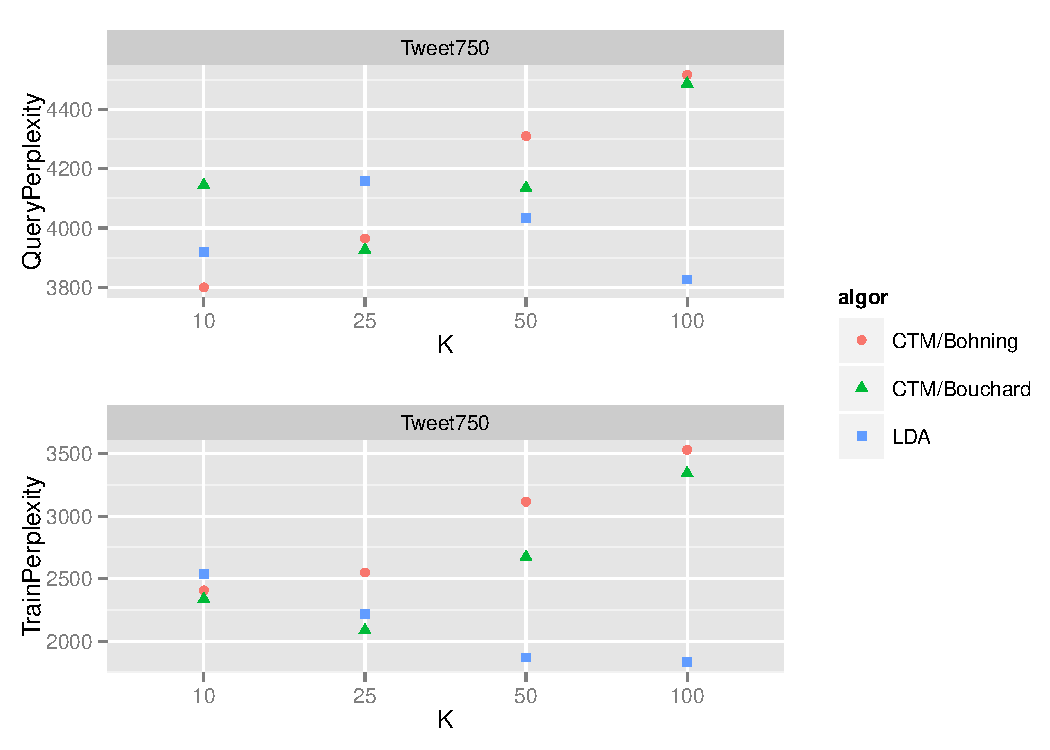
\includegraphics[width=0.7\textwidth]{plots/TweetCtmLda.pdf}
    \caption{Performance of LDA and CTM (implemented with Bohning and Bouchard bounds) on tweets aggregated by author}
    \label{fig:tweet-ctm-lda}
\end{figure}

\begin{figure}
\centering
    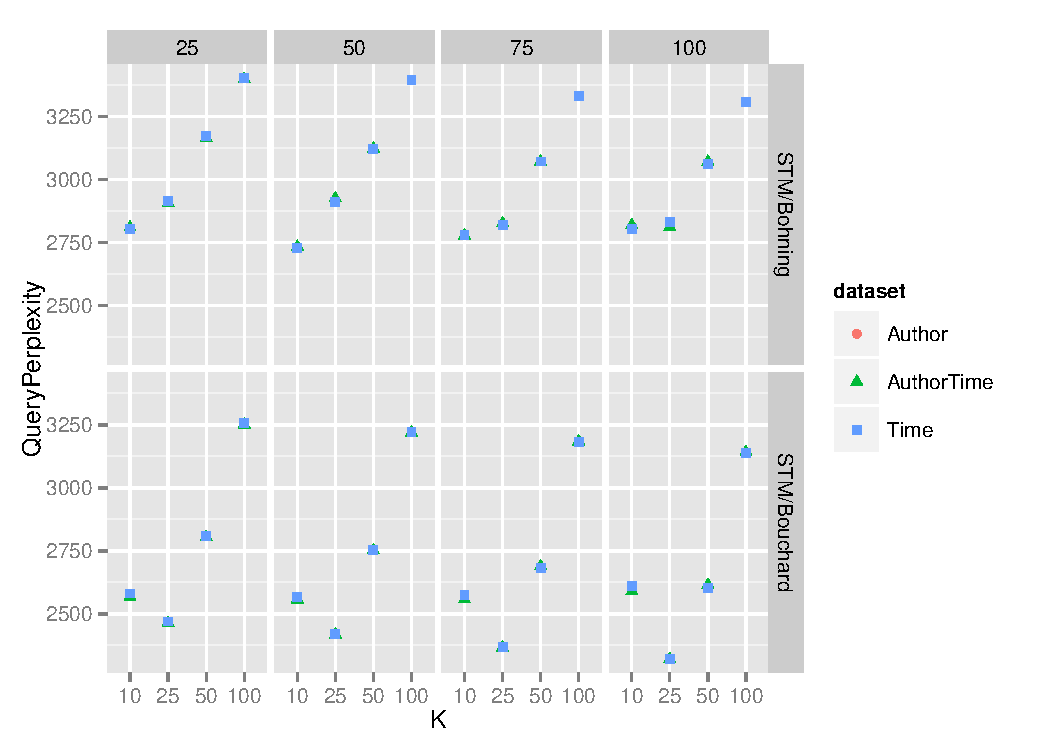
\includegraphics[width=0.8\textwidth]{plots/TweetStmQueryFeatures.pdf}
    \caption{Performance of the STM models depending on the chosen features, which were author only, author and time features, time features only}
    \label{fig:stm-p-all}
\end{figure}

\begin{table}
    \centering
    \begin{tabular}{| l || p{9cm} | } \hline 
        \bf{Hashtag} & %\bf{User (Internal)} & 
        \bf{Tweet Words} \\ \hline
        $\#$\tt{usopen} & %BreakPointBR & 
        Essa foi apenas a 2a vitoria de Gasquet nas oitavas de um Grand Slam. O frances alcanca sua primeira QFs em GS desde Wimbledon 2007 | \\ \hline
        $\#$\tt{f1} & %AustinGrandPrix & 
         MT @f1paddockpass: ...a big shout out to the marshalls \& volunteers here in Singapore. To all of you, heartfelt thanks @F1NightRace \\ \hline
        $\#$\tt{tcot} & %CraryAP & 
        $\#$Delaware Senate rejects bill to keep guns away from unstable people deemed danger to others http://hrld.us/110xnGt $\#$guncontrol $\#$NRA \\ \hline
        $\#$\tt{beer} & %Beer\_Disciples & 
        No-Li Brewhouse on track for 150\% growth, expanding annual capacity to 10,000 barrels ... \\ \hline
        $\#$\tt{obamacare} & %AFPhq & 
        @michellemalkin $\#$feded supporters simply believe you won't challenge them. $\#$stopcommoncore @afpne \\ \hline
        $\#$\tt{stones50} & %RollingStones & 
        Sweet Summer Sun - Hyde Park Live full length trailer! What do you think? http://www.youtube.com/watch?v=jgIXgYFUErE ... $\#$StonesHydePark \\ \hline
        $\#$\tt{eurozone} & %Annika\_Reuters & 
        $\#$German finmin $\#$Schaeuble argues $\#$Karlsruhe may have no jurisdiction over $\#$ECB measures.1st question by court's judges also focuses on this. \\ \hline
    \end{tabular}
    \caption{This table shows, for each hashtag, the tweet where that hashtag has the highest probability according to our model. The ``tcot" hashtag refers to ``true conservatives on twitter".}
    \label{tbl:generative}
\end{table}

\begin{figure}
\centering
    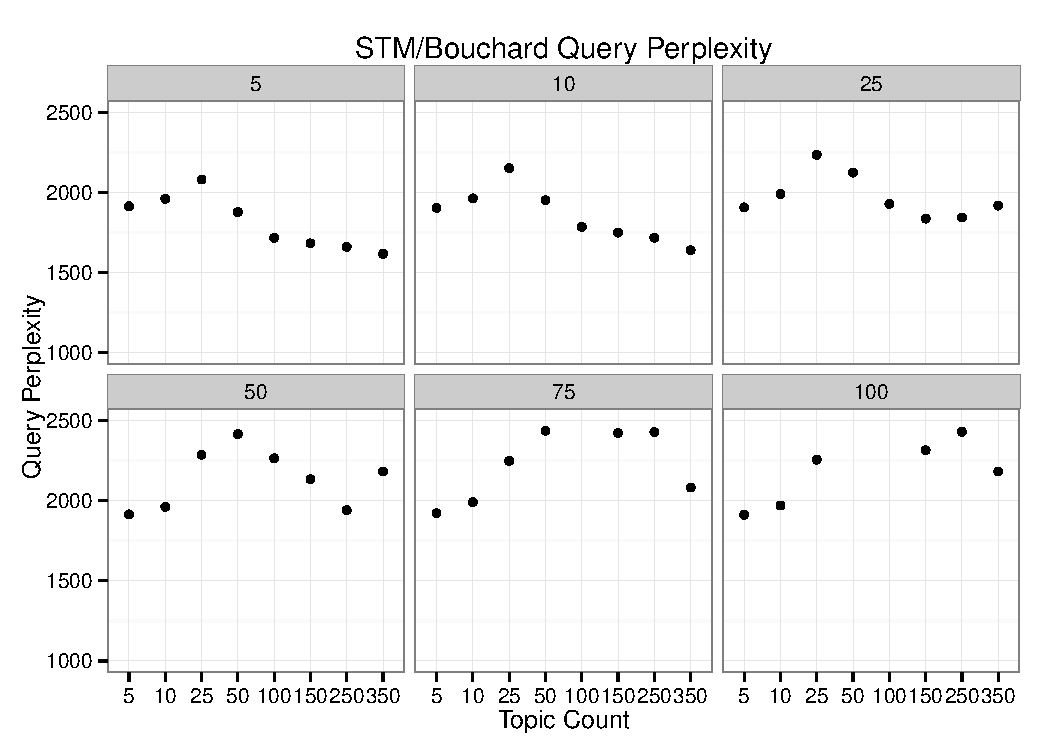
\includegraphics[width=0.8\textwidth]{plots/nips-stm-bou-kp.pdf}
    \caption{Performance of the STM models on NIPS datasets, using references and authors as features, implemented with the Bouchard bound}
    \label{fig:nips-stm-bou-p-all}
\end{figure}

\begin{figure}
\centering
    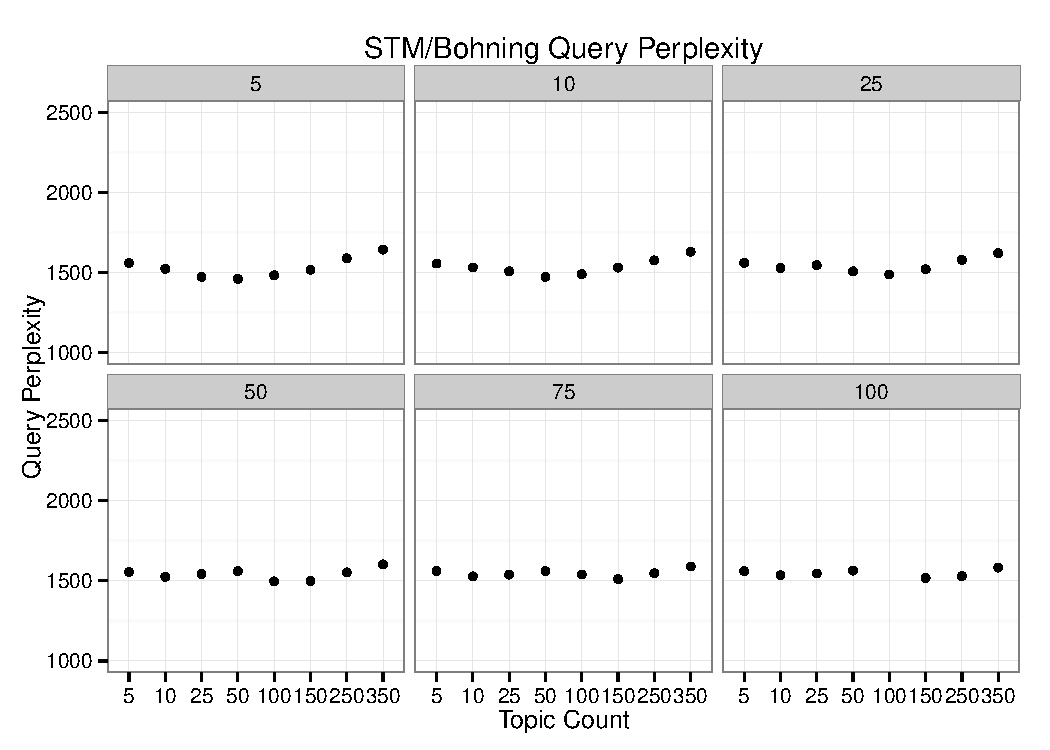
\includegraphics[width=0.8\textwidth]{plots/nips-stm-boh-kp.pdf}
    \caption{Performance of the STM models on NIPS datasets, using references and authors as features, implemented with the Bohning bound}
    \label{fig:nips-stm-boh-p-all}
\end{figure}

\begin{figure}
\centering
    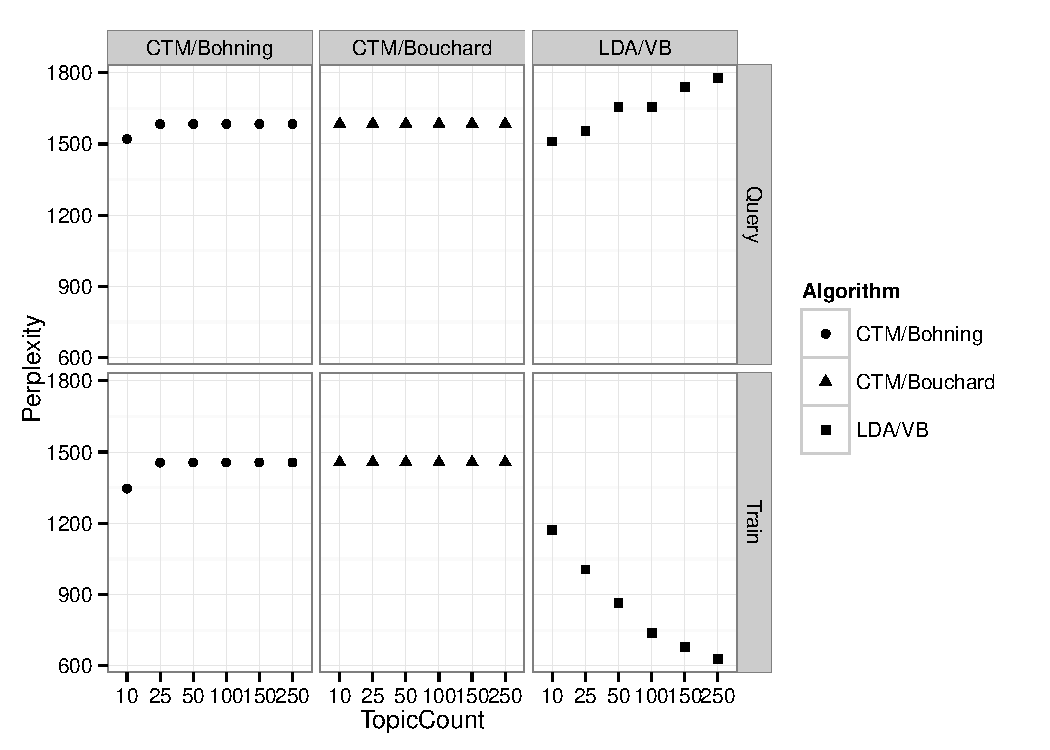
\includegraphics[width=0.8\textwidth]{plots/nips-lda-ctm.pdf}
    \caption{Performance of the CTM and LDA models on NIPS datasets}
    \label{fig:nips-lda-ctm}
\end{figure}



With regards to the choice of bound for the full-covariance model, the Bohning implementation is superior. One explanation of this could be that the Bohning approach allows us to calculate a full covariance matrix. However if we look at the results for individual users (see figure \ref{fig:bohing-bouchard-assignments}) we can see that when using the Bouchard bound, the algorithm essentially degenerates into a mixture model, as the posterior variances around the topic means approaches zero. 


Regardless of the algorithm chosen however, one issue which standards out is that the choice of the dimension of the latent feature-space, $P$, does not appear to affect results, suggesting that there is no correlation between features which can be exploited.



\subsubsection*{NIPS}
In the NIPS datasets the size of the latent dimension does have an effect on perplexity, though only in the case of the Bouchard bound (compare figure \ref{fig:nips-stm-bou-p-all} with figure \ref{fig:nips-stm-boh-p-all}). Looking at the training data in figure, we can see that as the number of topics increases, P also needs to increase as well to minimise perplexity, but only for the Bouchard bound (which again is essentially a mixture model).


\begin{figure}
\centering     %%% not \center
\subfigure[NIPS]{\label{fig:a}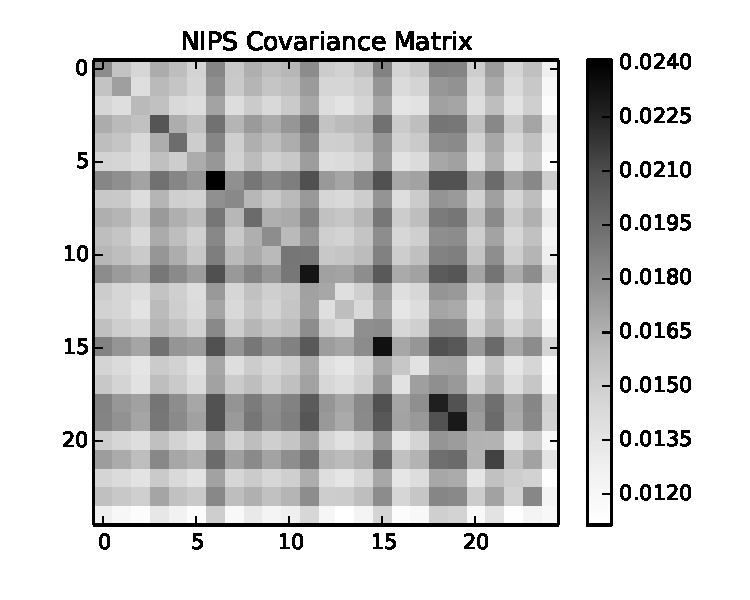
\includegraphics[width=60mm]{plots/nips-cov-k50-k50-boh.pdf}}
\subfigure[Tweets]{\label{fig:b}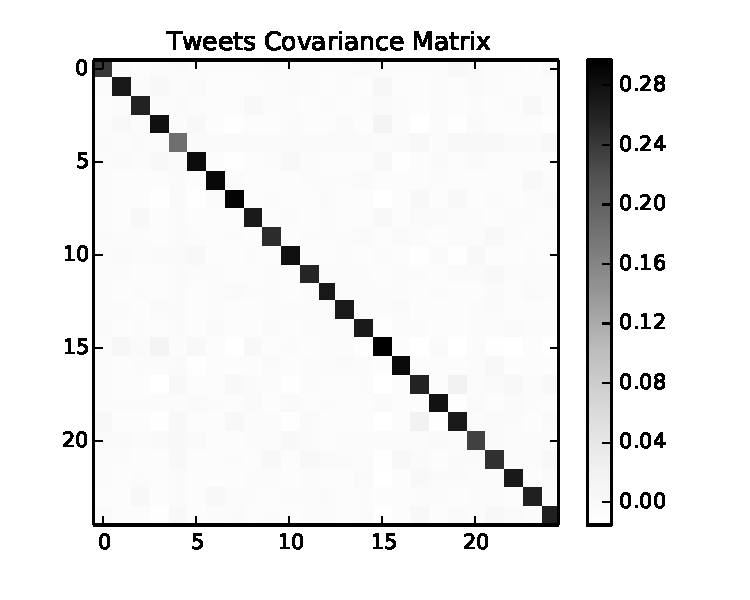
\includegraphics[width=60mm]{plots/tweets-cov-k50-k50-boh.pdf}}
\caption{Covariances over topics inferred using the Bohning implementation of the STM/YV model}
\end{figure}

\subsection{Conclusion}
In this paper we have introduced a method employing multi-task learning to predict admixture-components, using quadratic bounds to overcome the non-conjugacy of the model. We have successfully applied this method in the case of a dataset of tweets demonstrating better model fit versus a simple author topic model, and the ability to generate additional text that may help in query expansion. Our method is not specific to any particularly dataset, and so can be applied to any dataset where features may be associated with observations which can be fit using an admixture model.


%\begin{appendices}
%\section{The Variational Lower Bound}
%In this section we provide the variational lower-bound, or free-energy, for the two algorithms. This is taken after the bound has been applies to the likelihood.
%
%\subsection{Full-Covariance Model}
%The free-energy of the full-covariance bound is the sum of the terms given below.
%\begin{align}
%\begin{split}
%\ex{\ln p(Y)}{q} = &\halve{KP} \ln 2\pi - \halve{P}\ln |\Sigma| - \halve{KP}\ln \rho^2 - \half \Tr{\rho^{-2} \inv{\Sigma} M_Y M_Y\T}
%& \qquad + \half \Tr{S_Y\inv{\Sigma}\otimes R_Y \inv(\rho^{-2}I_P)}
%\end{split}
%\end{align}



%\section{Matrix Calculus Involving Kronecker Products}
%This briefly summarises the identities contained in three online resources\footnote{\url{http://research.microsoft.com/en-us/um/people/minka/papers/matrix/}}\footnote{\url{http://www4.ncsu.edu/~pfackler/MatCalc.pdf}}\footnote{\url{http://courses.engr.illinois.edu/cs598ps/CS598PS/Topics_and_Materials_files/Lecture\%201\%20-\%20Intro,\%20Linear\%20Algebra.pdf}} and then explains how these were used to take the derivatives of the expression
%
%\begin{equation}
%\Tr{A(X\T X \otimes Y\T Y) B}
%\end{equation}
%
%with respect to X and to Y.
%
%\subsection{Background}
%The definition of the Kronecker product and the $\vecf{\cdot}$ operator are assumed to be known. It is noted that in implementation terms, one can trivially implement the $\vecf{\cdot}$ operator using a \texttt{reshape} command, though only if the matrix is stored in column or ``Fortran" order. This is the case for Matlab, but most other numeric packages, including Numpy for Python, assume row or ``C" order. 
%
%Standard identites for Kronecker products and the related $\vecf{\cdot}$ operator are readily available\footnote{See for example ``The Matrix Cookbook" at \url{http://www2.imm.dtu.dk/pubdb/views/edoc_download.php/3274/pdf/imm3274.pdf}} but two of note are
%\begin{align}
%(X \otimes Y)\T & = X\T \otimes Y\T  \label{eqn:otimes_tranpose}\\
%\vecf{UXV} & = (V\T \otimes U)\vecf{X} \label{eqn:vec_to_otimes}
%\end{align}
%
%\subsubsection{The Vec-Transpose Operator}
%Both the $\vecf{\cdot}$ and tranpose operators can be generalized by the vec-transpose operator, introduced in \cite{Wandell1992}. This becomes a necessary tool when taking the derivatives of terms that occur in kronecker products.
%
%The vec-transpose of an $m \times n$ matrix $X$ is denoted $\vt{X}{p}$. The resulting matrix is composed of $n$ submatrices stacked atop one another, where each $p \times ^m/_p$ sub-matrix is generated by a fortran-order reshape of each column of X. The matrices are generated from top to bottom from the columns of X read from left to right. This is illustrated in the following examples.
%
%\begin{align}
%\begin{bmatrix} 
%    \color{Lavender}x_{11} & \color{CornflowerBlue}x_{12} \\
%    \color{Lavender}x_{21} & \color{CornflowerBlue}x_{22} \\
%    \color{Thistle}x_{31} & \color{RoyalBlue}x_{32} \\
%    \color{Thistle}x_{41} & \color{RoyalBlue}x_{42} \\
%    \color{Orchid}x_{51} & \color{Blue}x_{52} \\
%    \color{Orchid}x_{61} & \color{Blue}x_{62} 
%\end{bmatrix}^{(2)}
%= 
%\begin{bmatrix} 
%    \color{Lavender}x_{11} & \color{Thistle}x_{31} & \color{Orchid}x_{51} \\
%    \color{Lavender}x_{21} & \color{Thistle}x_{41} & \color{Orchid}x_{61} \\
%    \color{CornflowerBlue}x_{12} & \color{RoyalBlue}x_{32} & \color{Blue}x_{52} \\
%    \color{CornflowerBlue}x_{22} & \color{RoyalBlue}x_{42} & \color{Blue}x_{62} \\
%\end{bmatrix} \label{eqn:vt_example_2}
%\end{align}
%
%\begin{align}
%\begin{bmatrix} 
%    \color{Lavender}x_{11} & \color{CornflowerBlue}x_{12} \\
%    \color{Lavender}x_{21} & \color{CornflowerBlue}x_{22} \\
%    \color{Lavender}x_{31} & \color{CornflowerBlue}x_{32} \\
%    \color{Orchid}x_{41} & \color{NavyBlue}x_{42} \\
%    \color{Orchid}x_{51} & \color{NavyBlue}x_{52} \\
%    \color{Orchid}x_{61} & \color{NavyBlue}x_{62} 
%\end{bmatrix}^{(3)}
%= 
%\begin{bmatrix}
%    \color{Lavender}x_{11} & \color{Orchid}x_{41} \\
%    \color{Lavender}x_{21} & \color{Orchid}x_{51} \\
%    \color{Lavender}x_{31} & \color{Orchid}x_{61} \\
%    \color{CornflowerBlue}x_{12} & \color{NavyBlue}x_{42} \\
%    \color{CornflowerBlue}x_{22} & \color{NavyBlue}x_{52} \\
%    \color{CornflowerBlue}x_{32} & \color{NavyBlue}x_{62}
%\end{bmatrix}
%\end{align}
%
%The properties of the vec-transpose operator are:
%
%\begin{align}
%\vt{X}{1} & = X\T \\
%\vt{X}{\text{rows}(X)} & = \vecf{X} \\
%\vt{\vecf{X}}{r} & = \text{reshape(X,r,c)} & \text{\emph{(Fortran-order implementation)}} \\
%\vt{\vt{X}{p}}{p} & = X \label{eqn:a_pp_is_a} \\
%\vt{(aX + bY)}{p} & = a\vt{X}{p} + b\vt{Y}{p}
%\end{align}
%
%When working with traces, we can apply the vec-transpose operator inside the trace without affecting the result
%\begin{align}
%\Tr{X\T Y} = \Tr{\vt{(X)}{p}\T \vt{Y}{q}}
%\end{align}
%which generalizes the more commonly known identities
%\begin{align}
%\Tr{X\T Y} & = \vecf{X}\T\vecf{Y} \\
%\Tr{X\T Y} & = \Tr{X Y\T}
%\end{align}
%
%and in general we can apply any conformant reshaping, denoted with a a star, of the matrix dot-product within a trace without affecting the result
%\begin{align}
%\Tr{X\T Y} = \Tr{(X^*)\T Y^*} \label{eqn:tr_reshape}
%\end{align}
%
%{\color{red}An unproven result, verified empirically, is that for any matrix $X$ and appropriate values of $p$
%\begin{equation}
%    \left(\vt{X}{p}\right)\T \vt{I}{p} = \left(\vt{I}{p}\right)\T \vt{X}{p} \label{eqn:dot_of_vt_of_symmetric}
%\end{equation}
%}
%
%
%With these results in hand we can generalize equation \eqref{eqn:otimes_tranpose} as
%\begin{equation}
%\vt{(X \otimes Y)}{p} = X\T \otimes \vt{Y}{p} \label{eqn:vt_of_otimes}
%\end{equation}
%and equation \eqref{eqn:vec_to_otimes} as
%\begin{equation}
%\vt{\left((Z\T \otimes W)XY \right)}{p} = (Y \otimes W)\vt{X}{p}Z \label{eqn:extract_left_kro_opnd}
%\end{equation}
%where $p = \text{cols}(W)$.
%
%Crucially, this allows us to move the left operand, in this case $Z$, out of the kronecker product, enabling the use of standard identities to derive the derivative with respect to that operand.
%
%Using \eqref{eqn:extract_left_kro_opnd} we can show that
%\begin{equation}
%\vt{(\vt{(XY)}{p}Z)}{p} = (Z\T \otimes I)XY = \vt{(\vt{X}{p}Z)}{p}Y
%\end{equation}
%
%\subsubsection{The Commutation Matrix}
%In the previous section, we illustrated how we can swap-out the left-hand operand of a Kronecker product, enabling us to then apply the standard matrix-calculus identities. In this section we introduce the commutation matrix introduced in \cite{Magnus1988}, which allows us to swap the order of the operands in a kronecker product, moving the right-hand operand to the left from whence it can be swapped out subsequently using the vec-transpose operator.
%
%For an $m \times n$ matrix X, define the square matrix $T_{mn} \in \{0,1\}^{(m \times n) \times (m \times n)}$ that transforms $\vecf{X}$ into $\vecf{X\T}$:
%\begin{equation}
%T_{mn} \vecf{X} = \vecf{X\T}
%\end{equation}
%
%We can further define the matix $T_{nm}$ (note the order of the subscripts) such that
%\begin{align}
%T_{nm} T_{mn} \vecf{X}  & = \vecf{X} 
%\end{align}
%form which we can deduce the following three identities
%\begin{align}
%T_{nm} T_{mn}           &= I_{mn} \\
%T_{nm}                  &= \inv{T_{mn}} \\
%T_{mn}                  &= T_{nm}\T \label{eqn:transform_transpose}
%\end{align}
%
%Which taken together indicates that $T_{mn}$ is a square, orthogonal matrix. 
%
%These operators can be used to reorder the elements in a transpose. Assume X is an $m \times n$ matrix as before, and Y is a $k \times l$ matrix. Then
%\begin{align}
%Y \otimes X & = T_{km} (X \otimes Y) T_{nl} \label{eqn:kro_reorder} \\
%(X \otimes Y)T_{nl} & = T_{mk} (Y \otimes X)
%\end{align}
%Again, attention should be paid to the order of subscripts in the above results.
%
%Finally note that $T_{1m} = T_{m1} = I_m$. Hence, if for example X is a $1 \times n$ matrix then
%\begin{equation}
%(X \otimes Y)T_{nl} = Y \otimes X
%\end{equation}
%
%The elements of $T_{mn}$ are identified by the following equation, where $i \in [1\ldots mn]$ and $j \in [1 \ldots mn]$ are the row and column indices.
%\begin{equation}
%T_{mn}[i,j] = 
%\left\{
%    \begin{array}{lr}
%    1 & \text{if }  \left(j - \ceil{\frac{n}{i}}\right) \bmod n = 0 \\
%    0 & \text{otherwise}
%    \end{array}
%\right.
%\end{equation}
%
%
%\subsection{Connections between the Vec-Transpose Operator and Commutation Matrix}
%Looking at equation \eqref{eqn:vt_example_2}, where the vec-transform operator converts a $6 \times 2$ matrix into a $4 \times 3$ matrix, it is clear that no combination of square transformation matrices could achieve such a change in dimension, regardless of element ordering. Moreover $T_{mn}$ is explicitly defined in terms of the transform from $\vecf{X}$ to $\vecf{X\T}$
%
%Therefore rather than consider if one can express the vector-transform operator using commutation matrices, we must instead determine if a commutation matrix could be expressed in terms of the vec-transform operator.
%
%In short
%
%\begin{align}
%\mathcal{L}et\text{ } & \vv{x} = \vecf{X} & X \in \MReal{m}{n}\\
%\implies & T_{mn} \vv{x} = \vecf{X\T} \\
%\implies & T_{mn} \vv{x} = \vt{\vt{X}{1}}{n} \\
%\implies &\vt{\vt{\vt{\vv{x}}{m}}{1}}{n} = \vt{\vt{X}{1}}{n} \label{eqn:T_mn_to_vt}
%\end{align}
%
%Where in \eqref{eqn:T_mn_to_vt} we use \eqref{eqn:a_pp_is_a} to undo the $\vecf{\cdot}$ operation, then take the transpose via a vec-transpose operation, then re-apply $\vecf{\cdot}$ via another vec-transpose operation.
%
%Mathematically this is not a particularly useful result, replacing as it does one matrix multiplication with three applications of the vec-transpose operator. Programmatically, it is also likely that a sparse matrix-multiply is faster than several stacked \texttt{reshape} operations.
%
%\subsection{Derivatives of Terms in Kronecker Products}
%In this section we use the identities above, combined with standard matrix-calculus identities, to derive the derivative of
%
%\begin{equation}
%\Tr{A (X\T X \otimes Y\T Y) B}
%\end{equation}
%
%where $X \in \MReal{m}{n}$, $Y \in \MReal{k}{l}$, $A \in \MReal{nl}{a}$ and $B \in \MReal{nl}{b}$.
%
%\subsubsection{With Respect to the Left-Hand Operand}
%\newcommand \ddX  { \frac{d}{dX} }
%
%This proceeds in a straightforward manner, extending only slightly the example provided by Minka. 
%\begin{align}
%  & \ddX \Tr{A\T (X\T X \otimes Y\T Y) B} \\
%= & \ddX \Tr{\left(\vt{A}{l}\right)\T \vt{\left( (X\T X \otimes Y\T Y) B \right)}{l}} & \text{using } \eqref{eqn:tr_reshape} \\
%= & \ddX \Tr{\left(\vt{A}{l}\right)\T (I_{b} \otimes Y\T Y) \vt{B}{l} X\T X} & \text{using } \eqref{eqn:extract_left_kro_opnd} \\
%\begin{split}
%= & \quad X \left(\vt{A}{l}\right)\T (I_{b} \otimes Y\T Y) \vt{B}{l} \\
%  & \quad + X \left(\vt{B}{l}\right)\T (I_{b} \otimes Y\T Y) \vt{A}{l}  \label{eqn:lhs_kro_derivative}
%\end{split}
%\end{align}
%where in the final step we use the standard matrix-calculus result $\ddX \Tr{B X \T X} = XB + XB\T$. The scale of the vec-transporm operator is uniquely determined by conformability to be the number of columns in $Y\T Y$ which is $l$. If $A$ and $B$ are symmetric we can take advantage of \eqref{eqn:dot_of_vt_of_symmetric} to simplify the final result to
%\begin{equation}
%\ddX \Tr{A\T (X\T X \otimes Y\T Y) B} = 2X \left(\vt{A}{l}\right)\T (I_{b} \otimes Y\T Y) \vt{B}{l} \label{eqn:lhs_kro_derivative_symm_final}
%\end{equation}
%
%
%\subsubsection{With Respect to the Right-Hand Operand}
%This is much the same as before, except that we first employ two commutation matrices to re-arrange the order of the operands in the product.
%
%\begin{align}
%  & \ddX \Tr{A\T (X\T X \otimes Y\T Y ) B} \\
%= & \ddX \Tr{A\T T_{nl} (Y\T Y \otimes X\T X ) T_{ln} B} & \text{using }\eqref{eqn:kro_reorder} \\
%= & \ddX \Tr{ (T_{ln} A)\T (Y\T Y \otimes X\T X ) T_{ln} B} \text{using }\eqref{eqn:transform_transpose} \\
%= & \ddX \Tr{\left(\vt{(T_{ln} A)}{n}\right)\T \vt{\left( (Y\T Y \otimes X\T X ) T_{ln}B \right)}{n}} & \text{using } \eqref{eqn:tr_reshape} \\
%= & \ddX \Tr{\left(\vt{(T_{ln} A)}{n}\right)\T (I_b \otimes X\T X ) \vt{\left( T_{ln}B \right)}{n} Y\T Y } & \text{using } \eqref{eqn:extract_left_kro_opnd} \\
%\begin{split}
%= & \quad Y \left(\vt{(T_{ln} A)}{n}\right)\T (I_b \otimes X\T X ) \vt{\left( T_{ln}B \right)}{n} \\
%  & + Y \left(\vt{\left( T_{ln}B \right)}{n}\right)\T (I_b \otimes X\T X ) \vt{(T_{ln} A)}{n} \label{eqn:rhs_kro_derivative}
%\end{split}
%\end{align}
%
%The identity matrix in the kronecker produce is square with side equal to the columns of B. If B is square in turn, then the $I_b = I_{ln}$. {\color{red} TESTED BUT UNPROVEN. If A is symmetric and $B = I_{ln}$ then this simplifies to
%
%\begin{equation}
%\ddX \Tr{A\T (X\T X \otimes Y\T Y )} = 2 Y \left(\vt{(T_{ln} A)}{n}\right)\T (I_{ln} \otimes X\T X ) \vt{\left( T_{ln} \right)}{n} \label{eqn:rhs_kro_derivative_B_is_ident}
%\end{equation}
%}
%
%
%\end{appendices}
%



\bibliographystyle{plain}
\bibliography{/Users/bryanfeeney/Documents/library.bib}

\end{document}

